% Options for packages loaded elsewhere
\PassOptionsToPackage{unicode}{hyperref}
\PassOptionsToPackage{hyphens}{url}
%
\documentclass[
]{article}
\usepackage{lmodern}
\usepackage{amssymb,amsmath}
\usepackage{ifxetex,ifluatex}
\ifnum 0\ifxetex 1\fi\ifluatex 1\fi=0 % if pdftex
  \usepackage[T1]{fontenc}
  \usepackage[utf8]{inputenc}
  \usepackage{textcomp} % provide euro and other symbols
\else % if luatex or xetex
  \usepackage{unicode-math}
  \defaultfontfeatures{Scale=MatchLowercase}
  \defaultfontfeatures[\rmfamily]{Ligatures=TeX,Scale=1}
\fi
% Use upquote if available, for straight quotes in verbatim environments
\IfFileExists{upquote.sty}{\usepackage{upquote}}{}
\IfFileExists{microtype.sty}{% use microtype if available
  \usepackage[]{microtype}
  \UseMicrotypeSet[protrusion]{basicmath} % disable protrusion for tt fonts
}{}
\makeatletter
\@ifundefined{KOMAClassName}{% if non-KOMA class
  \IfFileExists{parskip.sty}{%
    \usepackage{parskip}
  }{% else
    \setlength{\parindent}{0pt}
    \setlength{\parskip}{6pt plus 2pt minus 1pt}}
}{% if KOMA class
  \KOMAoptions{parskip=half}}
\makeatother
\usepackage{xcolor}
\IfFileExists{xurl.sty}{\usepackage{xurl}}{} % add URL line breaks if available
\IfFileExists{bookmark.sty}{\usepackage{bookmark}}{\usepackage{hyperref}}
\hypersetup{
  pdftitle={PROJET 4a : le modèle SIR -- RMD},
  hidelinks,
  pdfcreator={LaTeX via pandoc}}
\urlstyle{same} % disable monospaced font for URLs
\usepackage[margin=1in]{geometry}
\usepackage{color}
\usepackage{fancyvrb}
\newcommand{\VerbBar}{|}
\newcommand{\VERB}{\Verb[commandchars=\\\{\}]}
\DefineVerbatimEnvironment{Highlighting}{Verbatim}{commandchars=\\\{\}}
% Add ',fontsize=\small' for more characters per line
\usepackage{framed}
\definecolor{shadecolor}{RGB}{248,248,248}
\newenvironment{Shaded}{\begin{snugshade}}{\end{snugshade}}
\newcommand{\AlertTok}[1]{\textcolor[rgb]{0.94,0.16,0.16}{#1}}
\newcommand{\AnnotationTok}[1]{\textcolor[rgb]{0.56,0.35,0.01}{\textbf{\textit{#1}}}}
\newcommand{\AttributeTok}[1]{\textcolor[rgb]{0.77,0.63,0.00}{#1}}
\newcommand{\BaseNTok}[1]{\textcolor[rgb]{0.00,0.00,0.81}{#1}}
\newcommand{\BuiltInTok}[1]{#1}
\newcommand{\CharTok}[1]{\textcolor[rgb]{0.31,0.60,0.02}{#1}}
\newcommand{\CommentTok}[1]{\textcolor[rgb]{0.56,0.35,0.01}{\textit{#1}}}
\newcommand{\CommentVarTok}[1]{\textcolor[rgb]{0.56,0.35,0.01}{\textbf{\textit{#1}}}}
\newcommand{\ConstantTok}[1]{\textcolor[rgb]{0.00,0.00,0.00}{#1}}
\newcommand{\ControlFlowTok}[1]{\textcolor[rgb]{0.13,0.29,0.53}{\textbf{#1}}}
\newcommand{\DataTypeTok}[1]{\textcolor[rgb]{0.13,0.29,0.53}{#1}}
\newcommand{\DecValTok}[1]{\textcolor[rgb]{0.00,0.00,0.81}{#1}}
\newcommand{\DocumentationTok}[1]{\textcolor[rgb]{0.56,0.35,0.01}{\textbf{\textit{#1}}}}
\newcommand{\ErrorTok}[1]{\textcolor[rgb]{0.64,0.00,0.00}{\textbf{#1}}}
\newcommand{\ExtensionTok}[1]{#1}
\newcommand{\FloatTok}[1]{\textcolor[rgb]{0.00,0.00,0.81}{#1}}
\newcommand{\FunctionTok}[1]{\textcolor[rgb]{0.00,0.00,0.00}{#1}}
\newcommand{\ImportTok}[1]{#1}
\newcommand{\InformationTok}[1]{\textcolor[rgb]{0.56,0.35,0.01}{\textbf{\textit{#1}}}}
\newcommand{\KeywordTok}[1]{\textcolor[rgb]{0.13,0.29,0.53}{\textbf{#1}}}
\newcommand{\NormalTok}[1]{#1}
\newcommand{\OperatorTok}[1]{\textcolor[rgb]{0.81,0.36,0.00}{\textbf{#1}}}
\newcommand{\OtherTok}[1]{\textcolor[rgb]{0.56,0.35,0.01}{#1}}
\newcommand{\PreprocessorTok}[1]{\textcolor[rgb]{0.56,0.35,0.01}{\textit{#1}}}
\newcommand{\RegionMarkerTok}[1]{#1}
\newcommand{\SpecialCharTok}[1]{\textcolor[rgb]{0.00,0.00,0.00}{#1}}
\newcommand{\SpecialStringTok}[1]{\textcolor[rgb]{0.31,0.60,0.02}{#1}}
\newcommand{\StringTok}[1]{\textcolor[rgb]{0.31,0.60,0.02}{#1}}
\newcommand{\VariableTok}[1]{\textcolor[rgb]{0.00,0.00,0.00}{#1}}
\newcommand{\VerbatimStringTok}[1]{\textcolor[rgb]{0.31,0.60,0.02}{#1}}
\newcommand{\WarningTok}[1]{\textcolor[rgb]{0.56,0.35,0.01}{\textbf{\textit{#1}}}}
\usepackage{longtable,booktabs}
% Correct order of tables after \paragraph or \subparagraph
\usepackage{etoolbox}
\makeatletter
\patchcmd\longtable{\par}{\if@noskipsec\mbox{}\fi\par}{}{}
\makeatother
% Allow footnotes in longtable head/foot
\IfFileExists{footnotehyper.sty}{\usepackage{footnotehyper}}{\usepackage{footnote}}
\makesavenoteenv{longtable}
\usepackage{graphicx,grffile}
\makeatletter
\def\maxwidth{\ifdim\Gin@nat@width>\linewidth\linewidth\else\Gin@nat@width\fi}
\def\maxheight{\ifdim\Gin@nat@height>\textheight\textheight\else\Gin@nat@height\fi}
\makeatother
% Scale images if necessary, so that they will not overflow the page
% margins by default, and it is still possible to overwrite the defaults
% using explicit options in \includegraphics[width, height, ...]{}
\setkeys{Gin}{width=\maxwidth,height=\maxheight,keepaspectratio}
% Set default figure placement to htbp
\makeatletter
\def\fps@figure{htbp}
\makeatother
\setlength{\emergencystretch}{3em} % prevent overfull lines
\providecommand{\tightlist}{%
  \setlength{\itemsep}{0pt}\setlength{\parskip}{0pt}}
\setcounter{secnumdepth}{-\maxdimen} % remove section numbering

\title{PROJET 4a : le modèle SIR -- RMD}
\author{}
\date{\vspace{-2.5em}13 décembre, 2020}

\begin{document}
\maketitle

\hypertarget{i.-consigne-et-objectifs}{%
\section{I. Consigne et objectifs}\label{i.-consigne-et-objectifs}}

Nous allons étudier une problématique biologique (au sens large) par des
simulations avec R.

Pour ce faire nous allons proposer:

\begin{itemize}
\item
  un code fonctionnel dans un package R
\item
  une présentation créée avec Rmarkdown
\item
  le partage du code et de la présentation avec github
\end{itemize}

Le projet que nous allons traiter est le \textbf{Projet 4 : le modèle
SIR}.

\hypertarget{ii.-ruxe9solution-du-projet}{%
\section{II. Résolution du projet}\label{ii.-ruxe9solution-du-projet}}

\hypertarget{pruxe9sentation-et-compruxe9hension-du-probluxe8me}{%
\subsubsection{1. Présentation et compréhension du
problème}\label{pruxe9sentation-et-compruxe9hension-du-probluxe8me}}

\hypertarget{le-moduxe8le-sir-dynamique-des-uxe9piduxe9mies}{%
\paragraph{1.1. Le Modèle SIR : dynamique des
épidémies}\label{le-moduxe8le-sir-dynamique-des-uxe9piduxe9mies}}

Le \textbf{modèle SIR} propose de représenter une épidémie en
compartimentant les individus d'une population N constante (on néglige
la natalité et la mortalité) en sous populations dynamiques au cours du
temps \emph{t} : \emph{sains} \textbf{\(S(t)\)}, \emph{infectés}
\textbf{\(I(t)\)} et \emph{retirés} \textbf{\(R(t)\)}. Dans ce modèle,
on considère les personnes retirées comme immunisées ou mortes, c'est
pourquoi on différentie les deux sous-populations \(S(t)\) et \(R(t)\).

Le modèle SIR est donc un modèle permettant de modeliser une épidémie,
c'est-à-dire de prédire la transmission d'un pathogène entre les
individus, les infections, et qu'il ne prend pas en compte la prédiction
de la mortalité de l'épidémie.

On sait que: \[N = S(t) + I(t) + R(t) = 1\]

Précisons que l'état du système à un instant t donné est défini par les
trois nombres \(S(t)\), \(I(t)\), \(R(t)\) sont des fractions de la
population et qu'on suppose qu'il y a beaucoup de personnes au sein
d'une population et qu'on peut donc oublier qu'on a des nombres entiers,
c'est-à-dire qu'il faudra considérer S,I et R comme des variables
continues.

Introduisons deux variables \(\beta\) et \(\gamma\) qui nous permettront
de définir le \textbf{taux de transmission \(\beta\)} et le \textbf{taux
de guérison \(\gamma\)}.

\[\beta\ \ \ \ \ \ \ \ \gamma\\  S  \longrightarrow I \longrightarrow  R  \]

Le taux de transmission \(\beta\) est donc le passage des personnes
saines à infectées et le taux de guérison \(\gamma\) est le passage des
personnes infectées à retirées.

\hypertarget{le-systuxe8me-duxe9quations-diffuxe9rentielles}{%
\paragraph{1.2. Le système d'équations
différentielles}\label{le-systuxe8me-duxe9quations-diffuxe9rentielles}}

Nous allons donc étudier l'évolution des sous populations en supposant
que la variation de \(S(t)\),\(I(t)\),\(R(t)\) à un instant donné t est
une fonction simple de la situation à ce même instant, c'est-à-dire que
l'évolution est régie par trois équations différentielles non linéaires
à trois inconnues.

Elles représentent un taux d'accroissement par rapport au temps :

\[\begin{equation}
    \left\{
     \begin{array}{l}
        S'(t) = \frac{dS(t)}{dt} = - \beta S(t)  I(t)\\
        I'(t) = \frac{dI(t)}{dt} = \beta S(t)  I(t) - \gamma  I(t)\\
        R'(t) = \frac{dR(t)}{dt} = \gamma I(t)
      \end{array}
    \right.
\end{equation}\]

De plus,on note : \[S'(t) + I'(t) + R'(t) = 0 \]

Ces 3 équations nous permettent d'obtenir des informations qualitatives
interressantes sur la façon dont l'épidémie se propage.

L'objectif du projet est d'estimer le temps du pic des infectés par des
simulations avec R.

\hypertarget{duxe9finition-du-coefficient-r0}{%
\paragraph{1.3. Définition du coefficient
R0}\label{duxe9finition-du-coefficient-r0}}

Dans notre étude, nous considérons que le nombre de personnes infectées
tend vers 0, c'est-à-dire que l'épidémie prend fin et les populations se
stabilisent.

Dans les conditions initiales, on donne S(0), I(0) et R(0) :

\begin{itemize}
\tightlist
\item
  \(0 \leqslant S(0)= s_0 \leqslant 1\) (valeur très proche de 1)
\item
  \(0 \leqslant I(0)= i_0 \leqslant 1\) (valeur très proche de 0)
\item
  \(R(0)= r_0 =0\) (on considère aucune personne guéries au début de
  l'épidémie)
\end{itemize}

A t=0 on peut écrire :

\[\begin{equation}
    \left\{
     \begin{array}{l}
        S'(0)  = - \beta S(0)  I(0)\\
        I'(0)  = \beta S(t)  I(0) - \gamma  I(0)\\
        R'(0)  =  \gamma I(0)
      \end{array}
    \right.
\end{equation}\]

Nous allons définir le \textbf{taux de reproduction \(R_0\)} comme le
nombre moyen de cas secondaires produits par un individu infectieux au
cours de sa période d'infection. La valeur que prend \(R_0\) determine
donc le nombre de personnes que va infecter une personne déja malade.

Reprenons l'équation 2 :

\[ I'(t) = \beta S(t)  I(t) - \gamma  I(t) \\= \gamma I (t)(\frac{\beta I(t) S(t)}{\gamma I(t)} -1) \\= \gamma I(t) (\frac{\beta  S(t)}{\gamma } -1) \\ =\gamma I(t) (R_0 S(t) -1)\]
On identifie \(R_0 = \frac{\beta}{\gamma}\) comme le \emph{coefficient
de contact}.

C'est ce coefficient là que les gouvernement tentent de maitriser lors
de la propagation d'une épidémie. Notamment avec les mesures de
confinement actuelles pour limiter le contact entre les personnes saines
et malades, et ainsi, réduire les contamminations.

Nous allons pouvoir evaluer le comportement de I'(t) grâce à ce
coefficient \(R_0\). En effet, nous savons que \(\gamma I\) est
forcément positif, donc c'est bien la valeur de \(R_0 S(t) - 1\) qui
determine le signe de \(\gamma I'(t)\).

\begin{itemize}
\tightlist
\item
  Si \(R_0 s_0 < 1\) alors \(I'(0) < 0\), ce qui veut dire que \(I(t)\)
  \emph{décroit}, l'épidémie prend fin.
\item
  Si \(R_0 s_0 > 1\) alors \(I'(0) > 0\), ce qui veut dire que \(I(t)\)
  \emph{croit}, et atteint une valeur maximale : c'est le \textbf{pic de
  l'épidemie}.
\end{itemize}

En effet, si un malade peut contaminer plus d'une personne (\(R_0 >1\))
la maladie va flamber.

\hypertarget{simulation-de-luxe9piduxe9mie-avec-r}{%
\subsubsection{2. Simulation de l'épidémie avec
R}\label{simulation-de-luxe9piduxe9mie-avec-r}}

\hypertarget{packages}{%
\paragraph{2.1. Packages}\label{packages}}

Installation du package crée pour ce projet :

\begin{Shaded}
\begin{Highlighting}[]
\CommentTok{#devtools::install_github("ZoeGerber/ModeleSIR")}
\KeywordTok{library}\NormalTok{(ModeleSIR)}
\end{Highlighting}
\end{Shaded}

Dans ce pakage ce trouve toutes les fonctions nécessaires pour réaliser
ces simulations du modèle SIR et prédire le pic des infectés.

Nous nous servirons également du package ggplot2 pour tracer nos courbes
:

\begin{Shaded}
\begin{Highlighting}[]
\KeywordTok{library}\NormalTok{(ggplot2)}
\end{Highlighting}
\end{Shaded}

\begin{verbatim}
## Warning: package 'ggplot2' was built under R version 4.0.3
\end{verbatim}

\hypertarget{ruxe9solution-du-systuxe8me-numuxe9riquement}{%
\paragraph{2.2. Résolution du système
numériquement}\label{ruxe9solution-du-systuxe8me-numuxe9riquement}}

On veut passer d'un modèle continu au discret.

Pendant une unité de temps \(\Delta t\), le nombre d'individus sains
passe de \(S(t)\) à \(S(t + \Delta t)\), et la variation de
\(S(t + \Delta t)–S(t)\) peut s'écrire :

\[\begin{equation}
    \left\{
     \begin{array}{l}
        \frac{dS(t)}{dt} = \frac{S(t + \Delta t)-S(t)}{\Delta t} \\
        \frac{dI(t)}{dt} = \frac{I(t + \Delta t) -I(t)}{\Delta t}  \\
        \frac{dS(t)}{dt} = \frac{R(t + \Delta t) -R(t)}{\Delta t} 
      \end{array}
    \right.
\end{equation}\]

Nous voulons isoler \(S(t + \Delta t)\) , \(I(t + \Delta t)\) et
\(R(t + \Delta t)\) afin de former une suite :

\[\begin{equation}
    \left\{
     \begin{array}{l}
        S(t + \Delta t) -S(t) = - \beta S(t)  I(t) \Delta t\\
        I(t + \Delta t) -I(t) = \beta S(t)  I(t) - \gamma  I(t) \Delta t\\
        R(t + \Delta t) -R(t) = \gamma I(t) \Delta t
      \end{array}
    \right.
\end{equation}\]

\[\begin{equation}
    \left\{
     \begin{array}{l}
        S(t + \Delta t)  = - \beta S(t)  I(t) \Delta t +S(t)\\
        I(t + \Delta t)  = [\beta S(t)  I(t) - \gamma  I(t)] \Delta t + I(t)\\
        R(t + \Delta t)  = \gamma I(t) \Delta t +R(t)
      \end{array}
    \right.
\end{equation}\]

Nous pouvons donc calculer les valeurs de S,I et R pour chaque valeurs
de t données, avec \(\Delta t\), fixé.

\hypertarget{calculs}{%
\paragraph{2.3. Calculs}\label{calculs}}

Si nous réalisions les calcul à la main nous pourrions donner le terme
suivant grâce au terme précédent, comme suit :

fixons pour l'exemple \(\beta = 0.5\), \(\gamma = 0.03\) et
\(\Delta t = 0.01\).

\begin{longtable}[]{@{}ccccccc@{}}
\toprule
\begin{minipage}[b]{0.05\columnwidth}\centering
t(j)\strut
\end{minipage} & \begin{minipage}[b]{0.11\columnwidth}\centering
S(t)\strut
\end{minipage} & \begin{minipage}[b]{0.11\columnwidth}\centering
I(t)\strut
\end{minipage} & \begin{minipage}[b]{0.11\columnwidth}\centering
R(t)\strut
\end{minipage} & \begin{minipage}[b]{0.16\columnwidth}\centering
S'(t)\strut
\end{minipage} & \begin{minipage}[b]{0.16\columnwidth}\centering
I'(t)\strut
\end{minipage} & \begin{minipage}[b]{0.11\columnwidth}\centering
R'(t)\strut
\end{minipage}\tabularnewline
\midrule
\endhead
\begin{minipage}[t]{0.05\columnwidth}\centering
0\strut
\end{minipage} & \begin{minipage}[t]{0.11\columnwidth}\centering
0.9\strut
\end{minipage} & \begin{minipage}[t]{0.11\columnwidth}\centering
0.1\strut
\end{minipage} & \begin{minipage}[t]{0.11\columnwidth}\centering
0\strut
\end{minipage} & \begin{minipage}[t]{0.16\columnwidth}\centering
-\(\beta\) * s0 * i0 = \textbf{-0.045}\strut
\end{minipage} & \begin{minipage}[t]{0.16\columnwidth}\centering
\(\beta\) * s0 * i0 - \(\gamma\) * i0 = \textbf{0.042}\strut
\end{minipage} & \begin{minipage}[t]{0.11\columnwidth}\centering
\(\gamma\) * i0 = \textbf{0.0003}\strut
\end{minipage}\tabularnewline
\begin{minipage}[t]{0.05\columnwidth}\centering
1\strut
\end{minipage} & \begin{minipage}[t]{0.11\columnwidth}\centering
s0-\(\beta\) * i0 * s0 * dt = \textbf{0.89955}\strut
\end{minipage} & \begin{minipage}[t]{0.11\columnwidth}\centering
i0+(\(\beta\) * i0 * s0 - \(\gamma\) * i0) * dt = \textbf{0.10042}\strut
\end{minipage} & \begin{minipage}[t]{0.11\columnwidth}\centering
0+ \(\gamma\) * i0 * dt = \textbf{3.10\^{}-5}\strut
\end{minipage} & \begin{minipage}[t]{0.16\columnwidth}\centering
\strut
\end{minipage} & \begin{minipage}[t]{0.16\columnwidth}\centering
\strut
\end{minipage} & \begin{minipage}[t]{0.11\columnwidth}\centering
\strut
\end{minipage}\tabularnewline
\begin{minipage}[t]{0.05\columnwidth}\centering
2\strut
\end{minipage} & \begin{minipage}[t]{0.11\columnwidth}\centering
\strut
\end{minipage} & \begin{minipage}[t]{0.11\columnwidth}\centering
\strut
\end{minipage} & \begin{minipage}[t]{0.11\columnwidth}\centering
\strut
\end{minipage} & \begin{minipage}[t]{0.16\columnwidth}\centering
\strut
\end{minipage} & \begin{minipage}[t]{0.16\columnwidth}\centering
\strut
\end{minipage} & \begin{minipage}[t]{0.11\columnwidth}\centering
\strut
\end{minipage}\tabularnewline
\begin{minipage}[t]{0.05\columnwidth}\centering
3\strut
\end{minipage} & \begin{minipage}[t]{0.11\columnwidth}\centering
\strut
\end{minipage} & \begin{minipage}[t]{0.11\columnwidth}\centering
\strut
\end{minipage} & \begin{minipage}[t]{0.11\columnwidth}\centering
\strut
\end{minipage} & \begin{minipage}[t]{0.16\columnwidth}\centering
\strut
\end{minipage} & \begin{minipage}[t]{0.16\columnwidth}\centering
\strut
\end{minipage} & \begin{minipage}[t]{0.11\columnwidth}\centering
\strut
\end{minipage}\tabularnewline
\bottomrule
\end{longtable}

Ce qui va nous interresser, c'est de pouvoir réaliser ces calcul avec R.

\hypertarget{initialisation}{%
\paragraph{2.4. Initialisation}\label{initialisation}}

Au début de l'épidémie (t=0) on a \(p\) personnes saines, et \(1-p\)
personnes infectées.

Il n'y a aucune personne retirées au début de l'épidémie.

\emph{\(p\)} est donc la proportion de personnes saines au commencement
de l'épidémie. (Cf fonction dans le package)

Les paramètres qui vont pouvoir être modifiés et ajustés au cours des
simulations sont :

\begin{itemize}
\tightlist
\item
  Le taux de transmission \(\beta\)
\item
  Le taux de guérison \(\gamma\)
\item
  Par extension de ces deux paramètres, le \(R_0\)
\item
  La proportion de personnes \(p\) saines au début de l'épidémie
\item
  La durée de la simulation (vecteur donné en jours)
\end{itemize}

\begin{enumerate}
\def\labelenumi{\alph{enumi}.}
\tightlist
\item
  Fractions initiales affichées (à t=0) de N qui sont Sains, Infectés et
  Retirés :
\end{enumerate}

\begin{Shaded}
\begin{Highlighting}[]
\KeywordTok{initSir}\NormalTok{(}\FloatTok{0.9}\NormalTok{)}
\end{Highlighting}
\end{Shaded}

\begin{verbatim}
## [1] 0.9 0.1 0.0
\end{verbatim}

\begin{enumerate}
\def\labelenumi{\alph{enumi}.}
\setcounter{enumi}{1}
\tightlist
\item
  Paramètres variables \(\beta\) et de \(\gamma\), qu'on suppose ne pas
  connaitre :
\end{enumerate}

Nous avons choisi de modéliser le \(R_0\) par une loi normale.

\begin{Shaded}
\begin{Highlighting}[]
\NormalTok{beta <-}\StringTok{ }\KeywordTok{tirageBeta}\NormalTok{(}\FloatTok{0.8}\NormalTok{,}\DecValTok{1}\NormalTok{)}
\KeywordTok{print}\NormalTok{(beta)}
\end{Highlighting}
\end{Shaded}

\begin{verbatim}
## [1] 1.449376
\end{verbatim}

\begin{Shaded}
\begin{Highlighting}[]
\NormalTok{gamma <-}\StringTok{ }\KeywordTok{tirageGamma}\NormalTok{(}\FloatTok{0.02}\NormalTok{,}\DecValTok{1}\NormalTok{)}
\KeywordTok{print}\NormalTok{(gamma)}
\end{Highlighting}
\end{Shaded}

\begin{verbatim}
## [1] 0.4632608
\end{verbatim}

\begin{Shaded}
\begin{Highlighting}[]
\NormalTok{R0 <-}\StringTok{ }\NormalTok{beta}\OperatorTok{/}\NormalTok{gamma}
\KeywordTok{print}\NormalTok{(R0)}
\end{Highlighting}
\end{Shaded}

\begin{verbatim}
## [1] 3.128641
\end{verbatim}

\hypertarget{courbes}{%
\paragraph{2.5 Courbes}\label{courbes}}

Pour cet exemple, choisissons :

\begin{itemize}
\tightlist
\item
  Taux de transmission \(\beta = 0.8\)
\item
  Taux de guérison \(\gamma=0.02\)
\item
  Proportion de personnes saines \(p=0.7888999\) au début de l'épidémie
\item
  Durée de la simulation : 50jours
\item
  \(\Delta t= 0.001\)
\end{itemize}

On part donc du \textbf{postulat} que le virus se transmet facilement,
et dont on guérit plutôt mal. La valeur du \(R_0\) est de 40.

\begin{Shaded}
\begin{Highlighting}[]
\NormalTok{df <-}\StringTok{ }\KeywordTok{sir}\NormalTok{(}\DecValTok{50}\NormalTok{,}\FloatTok{0.01}\NormalTok{,}\FloatTok{0.7888999}\NormalTok{,}\FloatTok{0.8}\NormalTok{,}\FloatTok{0.02}\NormalTok{)}

\KeywordTok{head}\NormalTok{(df)}
\end{Highlighting}
\end{Shaded}

\begin{verbatim}
##   j      resS      resI         resR
## 1 1 0.7888999 0.2111001 0.000000e+00
## 2 2 0.7875676 0.2123902 4.222002e-05
## 3 3 0.7862294 0.2136859 8.469805e-05
## 4 4 0.7848854 0.2149872 1.274352e-04
## 5 5 0.7835355 0.2162941 1.704327e-04
## 6 6 0.7821797 0.2176066 2.136915e-04
\end{verbatim}

\begin{Shaded}
\begin{Highlighting}[]
\KeywordTok{theme_set}\NormalTok{(}\KeywordTok{theme_minimal}\NormalTok{())}

\KeywordTok{ggplot}\NormalTok{(df, }\KeywordTok{aes}\NormalTok{(}\DataTypeTok{x=}\NormalTok{j)) }\OperatorTok{+}\StringTok{ }\KeywordTok{geom_line}\NormalTok{(}\KeywordTok{aes}\NormalTok{(}\DataTypeTok{y =}\NormalTok{ resS), }\DataTypeTok{color =} \StringTok{"darkgreen"}\NormalTok{) }\OperatorTok{+}\StringTok{ }\KeywordTok{geom_line}\NormalTok{(}\KeywordTok{aes}\NormalTok{(}\DataTypeTok{y =}\NormalTok{ resI),}\DataTypeTok{color =} \StringTok{"darkred"}\NormalTok{) }\OperatorTok{+}\StringTok{ }\KeywordTok{geom_line}\NormalTok{(}\KeywordTok{aes}\NormalTok{(}\DataTypeTok{y =}\NormalTok{ resR), }\DataTypeTok{color=}\StringTok{"steelblue"}\NormalTok{) }\OperatorTok{+}\StringTok{ }\KeywordTok{labs}\NormalTok{(}\DataTypeTok{title =} \StringTok{"Modèle SIR"}\NormalTok{, }\DataTypeTok{x =} \StringTok{"Temps"}\NormalTok{, }\DataTypeTok{y=}\StringTok{"Population"}\NormalTok{, }\DataTypeTok{color=}\StringTok{"L"}\NormalTok{) }\OperatorTok{+}\StringTok{ }\KeywordTok{labs}\NormalTok{(}\DataTypeTok{caption =} \StringTok{"Représentation graphique des populaions saines(en vert), infectées(en rouge) et guéries(en bleu)."}\NormalTok{)}\OperatorTok{+}\StringTok{ }\KeywordTok{theme}\NormalTok{(}\DataTypeTok{plot.caption =} \KeywordTok{element_text}\NormalTok{(}\DataTypeTok{hjust =} \FloatTok{0.5}\NormalTok{, }\DataTypeTok{face =} \StringTok{"italic"}\NormalTok{, }\DataTypeTok{size =}\DecValTok{10}\NormalTok{))}
\end{Highlighting}
\end{Shaded}

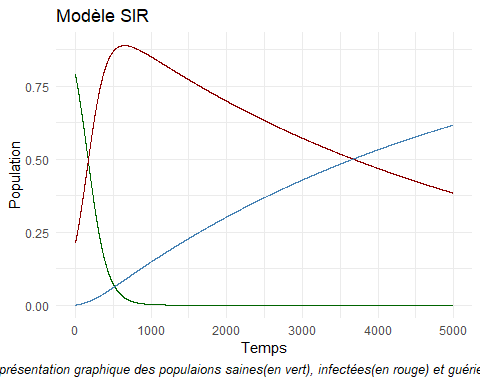
\includegraphics{Modele-SIR---RMD_files/figure-latex/unnamed-chunk-5-1.pdf}

En rouge la courbes des personnes \textbf{Infectées}, en bleu celle des
\textbf{Retirées} et en vert celle des personnes \textbf{Saines}

On observe que le pic de l'épidémie dans ces conditions fixées est haut
(quasiment toute la population a attrapé le virus (88,7\%)) et se touve
aux alentour du 10ème jour.Chaque personne malade contamine 40
personnes, ce qui est énorme.

Cherchons des pistes d'améliorations.

\hypertarget{simulations-et-analyses}{%
\subsection{3. Simulations et analyses}\label{simulations-et-analyses}}

Un fois notre graphe fonctionnel, nous pouvons donc nous amuser à
modifier la valeur des paramètres et ainsi ammener des premières
conclusions à ce modèle.

\hypertarget{taux-de-guuxe9rison-gamma}{%
\subsubsection{\texorpdfstring{3.1 Taux de guérison
\(\gamma\)}{3.1 Taux de guérison \textbackslash gamma}}\label{taux-de-guuxe9rison-gamma}}

\emph{Hypothèse 1} : Nous pouvons agir sur la guérison des personnes
malades (médicament ou système de santé performant par exemple)

Augmentons donc le taux de guérison \(\gamma\) :

\begin{itemize}
\tightlist
\item
  Taux de transmission \(\beta = 0.8\)
\item
  Taux de guérison \(\gamma=0.099\)
\item
  Proportion de personnes saines \(p=0.78885555\) au début de l'épidémie
\item
  Durée de la simulation : 50 jours
\item
  \(\Delta t= 0.01\)
\end{itemize}

\begin{Shaded}
\begin{Highlighting}[]
\NormalTok{df2 <-}\StringTok{ }\KeywordTok{sir}\NormalTok{(}\DecValTok{50}\NormalTok{,}\FloatTok{0.01}\NormalTok{,}\FloatTok{0.78885555}\NormalTok{,}\FloatTok{0.8}\NormalTok{,}\FloatTok{0.099}\NormalTok{)}
\KeywordTok{theme_set}\NormalTok{(}\KeywordTok{theme_minimal}\NormalTok{())}

\KeywordTok{ggplot}\NormalTok{(df2, }\KeywordTok{aes}\NormalTok{(}\DataTypeTok{x=}\NormalTok{j)) }\OperatorTok{+}\StringTok{ }\KeywordTok{geom_line}\NormalTok{(}\KeywordTok{aes}\NormalTok{(}\DataTypeTok{y =}\NormalTok{ resS), }\DataTypeTok{color =} \StringTok{"darkgreen"}\NormalTok{) }\OperatorTok{+}\StringTok{ }\KeywordTok{geom_line}\NormalTok{(}\KeywordTok{aes}\NormalTok{(}\DataTypeTok{y =}\NormalTok{ resI),}\DataTypeTok{color =} \StringTok{"darkred"}\NormalTok{) }\OperatorTok{+}\StringTok{ }\KeywordTok{geom_line}\NormalTok{(}\KeywordTok{aes}\NormalTok{(}\DataTypeTok{y =}\NormalTok{ resR), }\DataTypeTok{color=}\StringTok{"steelblue"}\NormalTok{) }\OperatorTok{+}\StringTok{ }\KeywordTok{labs}\NormalTok{(}\DataTypeTok{title =} \StringTok{"Modèle SIR"}\NormalTok{, }\DataTypeTok{x =} \StringTok{"Temps"}\NormalTok{, }\DataTypeTok{y=}\StringTok{"Population"}\NormalTok{, }\DataTypeTok{color=}\StringTok{"L"}\NormalTok{) }\OperatorTok{+}\StringTok{ }\KeywordTok{labs}\NormalTok{(}\DataTypeTok{caption =} \StringTok{"Représentation graphique des populaions saines(en vert), infectées(en rouge) et guéries(en bleu)."}\NormalTok{)}\OperatorTok{+}\StringTok{ }\KeywordTok{theme}\NormalTok{(}\DataTypeTok{plot.caption =} \KeywordTok{element_text}\NormalTok{(}\DataTypeTok{hjust =} \FloatTok{0.5}\NormalTok{, }\DataTypeTok{face =} \StringTok{"italic"}\NormalTok{, }\DataTypeTok{size =}\DecValTok{10}\NormalTok{))}
\end{Highlighting}
\end{Shaded}

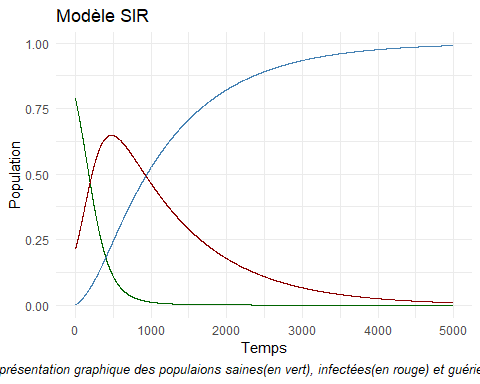
\includegraphics{Modele-SIR---RMD_files/figure-latex/unnamed-chunk-6-1.pdf}

On observe directement que le pic d'infectés est beaucoup moins haut (un
peu plus de 50\% (64,7\%) de la population à été malade), mais est
toujours au niveau du 10eme jour.

\hypertarget{taux-de-transmission-beta}{%
\subsubsection{\texorpdfstring{3.2 Taux de transmission
\(\beta\)}{3.2 Taux de transmission \textbackslash beta}}\label{taux-de-transmission-beta}}

\emph{Hypothèse 2} : Nous pouvons agir sur l'infection des personnes
saines (confinement, vaccin ou distantiacion sociale par exemple)

Diminuons donc le taux de transmission \(\beta\) :

\begin{itemize}
\tightlist
\item
  Taux de transmission \(\beta = 0.06\)
\item
  Taux de guérison \(\gamma=0.02\)
\item
  Proportion de personnes saines \(p=0.78885555\) au début de l'épidémie
\item
  Durée de la simulation : 50 jours
\item
  \(\Delta t= 0.01\)
\end{itemize}

\begin{Shaded}
\begin{Highlighting}[]
\NormalTok{df3 <-}\StringTok{ }\KeywordTok{sir}\NormalTok{(}\DecValTok{50}\NormalTok{,}\FloatTok{0.01}\NormalTok{,}\FloatTok{0.78885555}\NormalTok{,}\FloatTok{0.06}\NormalTok{,}\FloatTok{0.02}\NormalTok{)}
\KeywordTok{theme_set}\NormalTok{(}\KeywordTok{theme_minimal}\NormalTok{())}

\KeywordTok{ggplot}\NormalTok{(df3, }\KeywordTok{aes}\NormalTok{(}\DataTypeTok{x=}\NormalTok{j)) }\OperatorTok{+}\StringTok{ }\KeywordTok{geom_line}\NormalTok{(}\KeywordTok{aes}\NormalTok{(}\DataTypeTok{y =}\NormalTok{ resS), }\DataTypeTok{color =} \StringTok{"darkgreen"}\NormalTok{) }\OperatorTok{+}\StringTok{ }\KeywordTok{geom_line}\NormalTok{(}\KeywordTok{aes}\NormalTok{(}\DataTypeTok{y =}\NormalTok{ resI),}\DataTypeTok{color =} \StringTok{"darkred"}\NormalTok{) }\OperatorTok{+}\StringTok{ }\KeywordTok{geom_line}\NormalTok{(}\KeywordTok{aes}\NormalTok{(}\DataTypeTok{y =}\NormalTok{ resR), }\DataTypeTok{color=}\StringTok{"steelblue"}\NormalTok{) }\OperatorTok{+}\StringTok{ }\KeywordTok{labs}\NormalTok{(}\DataTypeTok{title =} \StringTok{"Modèle SIR"}\NormalTok{, }\DataTypeTok{x =} \StringTok{"Temps"}\NormalTok{, }\DataTypeTok{y=}\StringTok{"Population"}\NormalTok{, }\DataTypeTok{color=}\StringTok{"L"}\NormalTok{) }\OperatorTok{+}\StringTok{ }\KeywordTok{labs}\NormalTok{(}\DataTypeTok{caption =} \StringTok{"Représentation graphique des populaions saines(en vert), infectées(en rouge) et guéries(en bleu)."}\NormalTok{)}\OperatorTok{+}\StringTok{ }\KeywordTok{theme}\NormalTok{(}\DataTypeTok{plot.caption =} \KeywordTok{element_text}\NormalTok{(}\DataTypeTok{hjust =} \FloatTok{0.5}\NormalTok{, }\DataTypeTok{face =} \StringTok{"italic"}\NormalTok{, }\DataTypeTok{size =}\DecValTok{10}\NormalTok{))}
\end{Highlighting}
\end{Shaded}

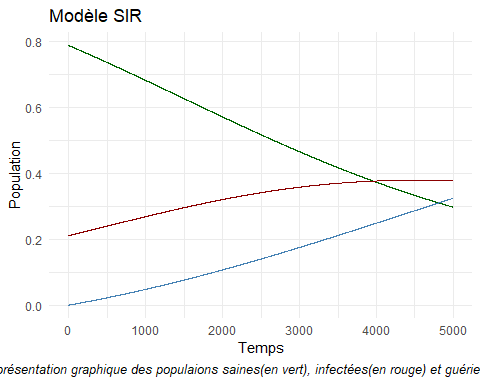
\includegraphics{Modele-SIR---RMD_files/figure-latex/unnamed-chunk-7-1.pdf}

On observe directement que le pic d'infectés est aussi moins haut , et
surtout plus étalé (certainement plus facile à gérer médicalement) : un
peu moins de 40\% (37.9\%) de la population à été malade. Il se trouve
au niveau du 50eme jour (ce qui laisse le temps de s'organiser pendant
une épidémie).

\hypertarget{taux-de-guuxe9rion-gamma-et-taux-de-transmission-beta}{%
\subsubsection{\texorpdfstring{3.3 Taux de guérion \(\gamma\) et taux de
transmission
\(\beta\)}{3.3 Taux de guérion \textbackslash gamma et taux de transmission \textbackslash beta}}\label{taux-de-guuxe9rion-gamma-et-taux-de-transmission-beta}}

\emph{Hypothèse 3} : Nous pouvons agir les deux paramètres en même
temps.

Diminuons donc le taux de transmission \(\beta\) et augmentons le taux
de guérion \(\gamma\) :

\begin{itemize}
\tightlist
\item
  Taux de transmission \(\beta = 0.06\)
\item
  Taux de guérison \(\gamma=0.099\)
\item
  Proportion de personnes saines \(p=0.78885555\) au début de l'épidémie
\item
  Durée de la simulation : 50jours
\item
  \(\Delta t= 0.01\)
\end{itemize}

\begin{Shaded}
\begin{Highlighting}[]
\NormalTok{df4 <-}\StringTok{ }\KeywordTok{sir}\NormalTok{(}\DecValTok{50}\NormalTok{,}\FloatTok{0.01}\NormalTok{,}\FloatTok{0.78885555}\NormalTok{,}\FloatTok{0.06}\NormalTok{,}\FloatTok{0.099}\NormalTok{)}
\KeywordTok{theme_set}\NormalTok{(}\KeywordTok{theme_minimal}\NormalTok{())}

\KeywordTok{ggplot}\NormalTok{(df4, }\KeywordTok{aes}\NormalTok{(}\DataTypeTok{x=}\NormalTok{j)) }\OperatorTok{+}\StringTok{ }\KeywordTok{geom_line}\NormalTok{(}\KeywordTok{aes}\NormalTok{(}\DataTypeTok{y =}\NormalTok{ resS), }\DataTypeTok{color =} \StringTok{"darkgreen"}\NormalTok{) }\OperatorTok{+}\StringTok{ }\KeywordTok{geom_line}\NormalTok{(}\KeywordTok{aes}\NormalTok{(}\DataTypeTok{y =}\NormalTok{ resI),}\DataTypeTok{color =} \StringTok{"darkred"}\NormalTok{) }\OperatorTok{+}\StringTok{ }\KeywordTok{geom_line}\NormalTok{(}\KeywordTok{aes}\NormalTok{(}\DataTypeTok{y =}\NormalTok{ resR), }\DataTypeTok{color=}\StringTok{"steelblue"}\NormalTok{) }\OperatorTok{+}\StringTok{ }\KeywordTok{labs}\NormalTok{(}\DataTypeTok{title =} \StringTok{"Modèle SIR"}\NormalTok{, }\DataTypeTok{x =} \StringTok{"Temps"}\NormalTok{, }\DataTypeTok{y=}\StringTok{"Population"}\NormalTok{, }\DataTypeTok{color=}\StringTok{"L"}\NormalTok{) }\OperatorTok{+}\StringTok{ }\KeywordTok{labs}\NormalTok{(}\DataTypeTok{caption =} \StringTok{"Représentation graphique des populaions saines(en vert), infectées(en rouge) et guéries(en bleu)."}\NormalTok{)}\OperatorTok{+}\StringTok{ }\KeywordTok{theme}\NormalTok{(}\DataTypeTok{plot.caption =} \KeywordTok{element_text}\NormalTok{(}\DataTypeTok{hjust =} \FloatTok{0.5}\NormalTok{, }\DataTypeTok{face =} \StringTok{"italic"}\NormalTok{, }\DataTypeTok{size =}\DecValTok{10}\NormalTok{)) }
\end{Highlighting}
\end{Shaded}

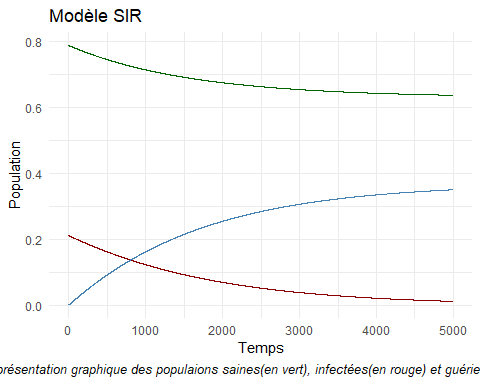
\includegraphics{Modele-SIR---RMD_files/figure-latex/unnamed-chunk-8-1.pdf}

\begin{Shaded}
\begin{Highlighting}[]
\KeywordTok{picI}\NormalTok{(}\FloatTok{0.06}\NormalTok{,}\FloatTok{0.099}\NormalTok{,df4)}
\end{Highlighting}
\end{Shaded}

\begin{verbatim}
##        PicI datePicI     R0pic
## 1 0.2111445        1 0.6060606
\end{verbatim}

On observe clairement que les mesures prises ont joué un role dans la
gestion de cette épidémie ! Certaines personnes n'ont même jamais
entendu parler de ce virus il semblerait ! Les personnes infectées
contaminaient moins de 1 personnes (0.6).

\hypertarget{iii.-ruxe9alisation-dune-uxe9tude-par-simulation-dune-quantituxe9-caractuxe9ristique}{%
\section{III. Réalisation d'une étude par simulation d'une quantité
caractéristique}\label{iii.-ruxe9alisation-dune-uxe9tude-par-simulation-dune-quantituxe9-caractuxe9ristique}}

Dans notre études précédente, nous avons modélisé différentes courbes
avec des valeurs du taux de reproduction \(R_0\) maitrisées, car on
donnait \(\beta\) et \(\gamma\).

En réalité, lors d'une épidémie, on ne connaît pas le \(R_0\)
précisément, et c'est lui qu'on cherche à determiner.

En effet, la connaissance précise du \(R_0\) nous permet de savoir s'il
faut prendre des mesures, et quand les prendre, comme imposer un
confinement (très restricif ou pas).

Reprenons des valeurs inconnues de \(\beta\) et \(\gamma\), et regardons
comment le \(R_0\) nous permet de prédire le pic.

Si on suppose \(R_0\) entre 2 bornes (\textgreater1 {[}pas d'épidémie{]}
et 20 {[}épidémie incontrôlée{]} par exemple), on pourra être capable de
déterminer la valeur du pic et le temps du pic.

\hypertarget{seuil-de-toluxe9rance-des-hopitaux}{%
\subsubsection{Seuil de tolérance des
hopitaux}\label{seuil-de-toluxe9rance-des-hopitaux}}

On cherche à avoir un pic d'infectés qui ne dépasse par une certaine
valeur (là où les hopitaux ne peuvent plus gérer les cas).

Avec des conditions initiales \(s0\) et \(i0\) données, on veut trouver
quand et de combien réduire le \(R_0\) pour éviter de dépasser ce seuil,
soit trouver quand imposer un confinement et de quelle nature (très
restricif ou peu restrictif)

Définissons arbitrairement notre seuil comme le moment ou les infectés
seraient à plus de 45\% de la population.

\begin{Shaded}
\begin{Highlighting}[]
\NormalTok{beta <-}\StringTok{ }\KeywordTok{tirageBeta}\NormalTok{(}\FloatTok{0.8}\NormalTok{,}\DecValTok{1}\NormalTok{)}
\KeywordTok{print}\NormalTok{(beta)}
\end{Highlighting}
\end{Shaded}

\begin{verbatim}
## [1] 1.292036
\end{verbatim}

\begin{Shaded}
\begin{Highlighting}[]
\NormalTok{gamma <-}\StringTok{ }\KeywordTok{tirageGamma}\NormalTok{(}\FloatTok{0.02}\NormalTok{,}\DecValTok{1}\NormalTok{)}
\KeywordTok{print}\NormalTok{(gamma)}
\end{Highlighting}
\end{Shaded}

\begin{verbatim}
## [1] 0.5483846
\end{verbatim}

\begin{Shaded}
\begin{Highlighting}[]
\NormalTok{R0 <-}\StringTok{ }\NormalTok{beta}\OperatorTok{/}\NormalTok{gamma}
\KeywordTok{print}\NormalTok{(R0)}
\end{Highlighting}
\end{Shaded}

\begin{verbatim}
## [1] 2.356077
\end{verbatim}

\begin{Shaded}
\begin{Highlighting}[]
\NormalTok{s <-}\StringTok{ }\KeywordTok{sir}\NormalTok{(}\DecValTok{50}\NormalTok{,}\FloatTok{0.1}\NormalTok{,}\FloatTok{0.7888999}\NormalTok{,beta,gamma)}
\KeywordTok{summary}\NormalTok{(s)}
\end{Highlighting}
\end{Shaded}

\begin{verbatim}
##        j              resS              resI                resR       
##  Min.   :  1.0   Min.   :0.08942   Min.   :0.0000000   Min.   :0.0000  
##  1st Qu.:125.8   1st Qu.:0.08942   1st Qu.:0.0000001   1st Qu.:0.9025  
##  Median :250.5   Median :0.08943   Median :0.0000255   Median :0.9105  
##  Mean   :250.5   Mean   :0.12009   Mean   :0.0332095   Mean   :0.8467  
##  3rd Qu.:375.2   3rd Qu.:0.09113   3rd Qu.:0.0063335   3rd Qu.:0.9106  
##  Max.   :500.0   Max.   :0.78890   Max.   :0.3172818   Max.   :0.9106
\end{verbatim}

\begin{Shaded}
\begin{Highlighting}[]
\KeywordTok{head}\NormalTok{(s)}
\end{Highlighting}
\end{Shaded}

\begin{verbatim}
##   j      resS      resI       resR
## 1 1 0.7888999 0.2111001 0.00000000
## 2 2 0.7673827 0.2210409 0.01157640
## 3 3 0.7454668 0.2308352 0.02369794
## 4 4 0.7232335 0.2404099 0.03635659
## 5 5 0.7007685 0.2496912 0.04954030
## 6 6 0.6781610 0.2586060 0.06323298
\end{verbatim}

\begin{Shaded}
\begin{Highlighting}[]
\KeywordTok{theme_set}\NormalTok{(}\KeywordTok{theme_minimal}\NormalTok{())}

\KeywordTok{ggplot}\NormalTok{(s, }\KeywordTok{aes}\NormalTok{(}\DataTypeTok{x=}\NormalTok{j)) }\OperatorTok{+}\StringTok{ }\KeywordTok{geom_line}\NormalTok{(}\KeywordTok{aes}\NormalTok{(}\DataTypeTok{y =}\NormalTok{ resS), }\DataTypeTok{color =} \StringTok{"darkgreen"}\NormalTok{) }\OperatorTok{+}\StringTok{ }\KeywordTok{geom_line}\NormalTok{(}\KeywordTok{aes}\NormalTok{(}\DataTypeTok{y =}\NormalTok{ resI),}\DataTypeTok{color =} \StringTok{"darkred"}\NormalTok{) }\OperatorTok{+}\StringTok{ }\KeywordTok{geom_line}\NormalTok{(}\KeywordTok{aes}\NormalTok{(}\DataTypeTok{y =}\NormalTok{ resR), }\DataTypeTok{color=}\StringTok{"steelblue"}\NormalTok{) }\OperatorTok{+}\StringTok{ }\KeywordTok{labs}\NormalTok{(}\DataTypeTok{title =} \StringTok{"Modèle SIR"}\NormalTok{, }\DataTypeTok{x =} \StringTok{"Temps"}\NormalTok{, }\DataTypeTok{y=}\StringTok{"Population"}\NormalTok{, }\DataTypeTok{color=}\StringTok{"L"}\NormalTok{) }\OperatorTok{+}\StringTok{ }\KeywordTok{labs}\NormalTok{(}\DataTypeTok{caption =} \StringTok{"Représentation graphique des populaions saines(en vert), infectées(en rouge) et guéries(en bleu)."}\NormalTok{)}\OperatorTok{+}\StringTok{ }\KeywordTok{theme}\NormalTok{(}\DataTypeTok{plot.caption =} \KeywordTok{element_text}\NormalTok{(}\DataTypeTok{hjust =} \FloatTok{0.5}\NormalTok{, }\DataTypeTok{face =} \StringTok{"italic"}\NormalTok{, }\DataTypeTok{size =}\DecValTok{10}\NormalTok{))}
\end{Highlighting}
\end{Shaded}

\includegraphics{Modele-SIR---RMD_files/figure-latex/unnamed-chunk-11-1.pdf}

\begin{Shaded}
\begin{Highlighting}[]
\NormalTok{p <-}\StringTok{ }\KeywordTok{picI}\NormalTok{(beta,gamma,s)}
\KeywordTok{print}\NormalTok{(p)}
\end{Highlighting}
\end{Shaded}

\begin{verbatim}
##        PicI datePicI    R0pic
## 1 0.3172818       19 2.356077
\end{verbatim}

\hypertarget{replicate}{%
\subsection{Replicate()}\label{replicate}}

\begin{Shaded}
\begin{Highlighting}[]
\NormalTok{list_res <-}\StringTok{ }\KeywordTok{data.frame}\NormalTok{(}\KeywordTok{replicate}\NormalTok{(}\DecValTok{50}\NormalTok{,}\KeywordTok{picI2}\NormalTok{(}\DecValTok{10}\NormalTok{,}\FloatTok{0.01}\NormalTok{,}\FloatTok{0.7888999}\NormalTok{,}\FloatTok{0.6}\NormalTok{,}\FloatTok{0.03}\NormalTok{,}\DecValTok{1}\NormalTok{,}\DecValTok{1}\NormalTok{), }\DataTypeTok{simplify=}\NormalTok{T))}
\KeywordTok{print}\NormalTok{(list_res)}
\end{Highlighting}
\end{Shaded}

\begin{verbatim}
##                 X1        X2        X3        X4         X5        X6        X7
## PicI     0.4540822 0.4566669 0.5441074 0.2111001  0.2111001 0.5510903 0.5479172
## datePicI       398      1000       198         1          1       154       833
## R0pic     3.876227  5.014139  5.332752   0.75414 0.02696213  5.466842  5.425005
##                 X8        X9       X10       X11       X12       X13       X14
## PicI     0.5125801 0.2111001 0.2111001 0.3624852 0.4164589 0.2111001 0.4688711
## datePicI       144         1         1       383       770         1       187
## R0pic     4.747516  0.660437 0.8932627  2.823423   3.40677 0.9684806  4.073448
##                X15       X16       X17       X18       X19      X20       X21
## PicI     0.5810233 0.3878727 0.2111001 0.2431636 0.2111001 0.314646 0.2111001
## datePicI       154       183         1       359         1      461         1
## R0pic     6.126295  3.080804  0.590965  1.738537 0.6331123 2.373984 0.7559629
##                X22       X23       X24       X25         X26       X27
## PicI     0.3244385 0.2111001 0.2111001 0.4380808   0.2111001 0.2111001
## datePicI       152         1         1       160           1         1
## R0pic     2.458842 0.1282153 0.8413413  3.660105 0.005402302 0.6633801
##                X28       X29       X30       X31       X32       X33       X34
## PicI     0.2111001 0.8966972 0.2111001 0.2251514 0.2405009 0.6854885 0.2111001
## datePicI         1       231         1        87       107      1000         1
## R0pic     1.117401  43.64614 0.4460611   1.54913  1.711178  12.38383 0.4854573
##                X35      X36       X37       X38       X39       X40       X41
## PicI     0.2111001 0.637224 0.2496684 0.2111001 0.2111001 0.6026953 0.2493341
## datePicI         1      277        86         1         1       304        62
## R0pic    0.5618483 7.718627   1.79665 0.4890378 0.8158498  6.692502  1.792122
##                X42       X43       X44       X45       X46       X47       X48
## PicI     0.2111001 0.4719396 0.2111001 0.2111001 0.2111001 0.9216675 0.4556216
## datePicI         1       447         1         1         1       393       217
## R0pic     1.036792  4.125225 0.5803379 0.6026972 0.4006998  62.19285   3.89214
##                X49       X50
## PicI     0.2795172 0.2111001
## datePicI       102         1
## R0pic     2.060914 0.9253907
\end{verbatim}

\begin{Shaded}
\begin{Highlighting}[]
\NormalTok{concat <-}\StringTok{ }\KeywordTok{do.call}\NormalTok{(rbind.data.frame,list_res)}
\KeywordTok{print}\NormalTok{(concat)}
\end{Highlighting}
\end{Shaded}

\begin{verbatim}
##          PicI datePicI        R0pic
## X1  0.4540822      398  3.876227389
## X2  0.4566669     1000  5.014139094
## X3  0.5441074      198  5.332751777
## X4  0.2111001        1  0.754139983
## X5  0.2111001        1  0.026962128
## X6  0.5510903      154  5.466842393
## X7  0.5479172      833  5.425004962
## X8  0.5125801      144  4.747515897
## X9  0.2111001        1  0.660437030
## X10 0.2111001        1  0.893262734
## X11 0.3624852      383  2.823422624
## X12 0.4164589      770  3.406769761
## X13 0.2111001        1  0.968480559
## X14 0.4688711      187  4.073448414
## X15 0.5810233      154  6.126295330
## X16 0.3878727      183  3.080803934
## X17 0.2111001        1  0.590965011
## X18 0.2431636      359  1.738536835
## X19 0.2111001        1  0.633112311
## X20 0.3146460      461  2.373983862
## X21 0.2111001        1  0.755962911
## X22 0.3244385      152  2.458841809
## X23 0.2111001        1  0.128215320
## X24 0.2111001        1  0.841341291
## X25 0.4380808      160  3.660104590
## X26 0.2111001        1  0.005402302
## X27 0.2111001        1  0.663380141
## X28 0.2111001        1  1.117401143
## X29 0.8966972      231 43.646141136
## X30 0.2111001        1  0.446061078
## X31 0.2251514       87  1.549129594
## X32 0.2405009      107  1.711177853
## X33 0.6854885     1000 12.383828262
## X34 0.2111001        1  0.485457264
## X35 0.2111001        1  0.561848325
## X36 0.6372240      277  7.718627062
## X37 0.2496684       86  1.796649774
## X38 0.2111001        1  0.489037767
## X39 0.2111001        1  0.815849837
## X40 0.6026953      304  6.692501791
## X41 0.2493341       62  1.792122469
## X42 0.2111001        1  1.036791859
## X43 0.4719396      447  4.125224995
## X44 0.2111001        1  0.580337851
## X45 0.2111001        1  0.602697231
## X46 0.2111001        1  0.400699798
## X47 0.9216675      393 62.192853133
## X48 0.4556216      217  3.892140154
## X49 0.2795172      102  2.060914475
## X50 0.2111001        1  0.925390691
\end{verbatim}

\begin{Shaded}
\begin{Highlighting}[]
\NormalTok{orderConcat <-}\StringTok{ }\NormalTok{concat[}\KeywordTok{order}\NormalTok{(concat[,}\DecValTok{3}\NormalTok{],}\DataTypeTok{decreasing=}\NormalTok{F),]}
\KeywordTok{print}\NormalTok{(orderConcat)}
\end{Highlighting}
\end{Shaded}

\begin{verbatim}
##          PicI datePicI        R0pic
## X26 0.2111001        1  0.005402302
## X5  0.2111001        1  0.026962128
## X23 0.2111001        1  0.128215320
## X46 0.2111001        1  0.400699798
## X30 0.2111001        1  0.446061078
## X34 0.2111001        1  0.485457264
## X38 0.2111001        1  0.489037767
## X35 0.2111001        1  0.561848325
## X44 0.2111001        1  0.580337851
## X17 0.2111001        1  0.590965011
## X45 0.2111001        1  0.602697231
## X19 0.2111001        1  0.633112311
## X9  0.2111001        1  0.660437030
## X27 0.2111001        1  0.663380141
## X4  0.2111001        1  0.754139983
## X21 0.2111001        1  0.755962911
## X39 0.2111001        1  0.815849837
## X24 0.2111001        1  0.841341291
## X10 0.2111001        1  0.893262734
## X50 0.2111001        1  0.925390691
## X13 0.2111001        1  0.968480559
## X42 0.2111001        1  1.036791859
## X28 0.2111001        1  1.117401143
## X31 0.2251514       87  1.549129594
## X32 0.2405009      107  1.711177853
## X18 0.2431636      359  1.738536835
## X41 0.2493341       62  1.792122469
## X37 0.2496684       86  1.796649774
## X49 0.2795172      102  2.060914475
## X20 0.3146460      461  2.373983862
## X22 0.3244385      152  2.458841809
## X11 0.3624852      383  2.823422624
## X16 0.3878727      183  3.080803934
## X12 0.4164589      770  3.406769761
## X25 0.4380808      160  3.660104590
## X1  0.4540822      398  3.876227389
## X48 0.4556216      217  3.892140154
## X14 0.4688711      187  4.073448414
## X43 0.4719396      447  4.125224995
## X8  0.5125801      144  4.747515897
## X2  0.4566669     1000  5.014139094
## X3  0.5441074      198  5.332751777
## X7  0.5479172      833  5.425004962
## X6  0.5510903      154  5.466842393
## X15 0.5810233      154  6.126295330
## X40 0.6026953      304  6.692501791
## X36 0.6372240      277  7.718627062
## X33 0.6854885     1000 12.383828262
## X29 0.8966972      231 43.646141136
## X47 0.9216675      393 62.192853133
\end{verbatim}

\begin{Shaded}
\begin{Highlighting}[]
\KeywordTok{ggplot}\NormalTok{(orderConcat, }\KeywordTok{aes}\NormalTok{(}\DataTypeTok{x =}\NormalTok{ R0pic)) }\OperatorTok{+}\StringTok{ }\KeywordTok{geom_line}\NormalTok{(}\KeywordTok{aes}\NormalTok{(}\DataTypeTok{y =}\NormalTok{ PicI), }\DataTypeTok{col=}\StringTok{"purple"}\NormalTok{)}\OperatorTok{+}\KeywordTok{geom_line}\NormalTok{(}\KeywordTok{aes}\NormalTok{(}\DataTypeTok{y =} \FloatTok{0.45}\NormalTok{), }\DataTypeTok{col=}\StringTok{"red"}\NormalTok{, }\DataTypeTok{linetype =} \StringTok{"dashed"}\NormalTok{, }\DataTypeTok{size=}\DecValTok{2}\NormalTok{)}\OperatorTok{+}\StringTok{ }\KeywordTok{labs}\NormalTok{(}\DataTypeTok{title =} \StringTok{"Valeur du pic en focntion du R0"}\NormalTok{, }\DataTypeTok{x =} \StringTok{"R0"}\NormalTok{, }\DataTypeTok{y=}\StringTok{"Pic des infectés"}\NormalTok{, }\DataTypeTok{color=}\StringTok{"red"}\NormalTok{) }\OperatorTok{+}\StringTok{ }\KeywordTok{labs}\NormalTok{(}\DataTypeTok{caption =} \StringTok{"Représentation graphique des valeurs des pics à différents R0"}\NormalTok{)}\OperatorTok{+}\StringTok{ }\KeywordTok{theme}\NormalTok{(}\DataTypeTok{plot.caption =} \KeywordTok{element_text}\NormalTok{(}\DataTypeTok{hjust =} \FloatTok{0.5}\NormalTok{, }\DataTypeTok{face =} \StringTok{"italic"}\NormalTok{, }\DataTypeTok{size =}\DecValTok{10}\NormalTok{))}
\end{Highlighting}
\end{Shaded}

\includegraphics{Modele-SIR---RMD_files/figure-latex/unnamed-chunk-14-1.pdf}

\begin{Shaded}
\begin{Highlighting}[]
 \KeywordTok{ggplot}\NormalTok{(orderConcat, }\KeywordTok{aes}\NormalTok{(}\DataTypeTok{x =}\NormalTok{ R0pic)) }\OperatorTok{+}\StringTok{ }\KeywordTok{geom_line}\NormalTok{(}\KeywordTok{aes}\NormalTok{(}\DataTypeTok{y =}\NormalTok{ datePicI), }\DataTypeTok{col=}\StringTok{"purple"}\NormalTok{)}\OperatorTok{+}\StringTok{ }\KeywordTok{labs}\NormalTok{(}\DataTypeTok{title =} \StringTok{"Date du pic en focntion du R0"}\NormalTok{, }\DataTypeTok{x =} \StringTok{"R0"}\NormalTok{, }\DataTypeTok{y=}\StringTok{"Dates des pics des infectés"}\NormalTok{, }\DataTypeTok{color=}\StringTok{"red"}\NormalTok{) }\OperatorTok{+}\StringTok{ }\KeywordTok{labs}\NormalTok{(}\DataTypeTok{caption =} \StringTok{"Représentation graphique des valeurs des pics à différents R0"}\NormalTok{)}\OperatorTok{+}\StringTok{ }\KeywordTok{theme}\NormalTok{(}\DataTypeTok{plot.caption =} \KeywordTok{element_text}\NormalTok{(}\DataTypeTok{hjust =} \FloatTok{0.5}\NormalTok{, }\DataTypeTok{face =} \StringTok{"italic"}\NormalTok{, }\DataTypeTok{size =}\DecValTok{10}\NormalTok{))}
\end{Highlighting}
\end{Shaded}

\includegraphics{Modele-SIR---RMD_files/figure-latex/unnamed-chunk-14-2.pdf}

A partir de quelle valeur du \(R_0\) les hopitaux sont-ils débordés ?

\hypertarget{iv.-complexification-et-ruxe9alisme-du-moduxe8le-sir}{%
\section{IV. Complexification et réalisme du modèle
SIR}\label{iv.-complexification-et-ruxe9alisme-du-moduxe8le-sir}}

\hypertarget{ruxe9alisme}{%
\subsubsection{1. Réalisme}\label{ruxe9alisme}}

Le modèle SIR est un modèle simple, qui considèrait une population
constante au cours du temps, où les naissances et la mortalité étaient
négilgées.

En effet, pour se rapprocher de la réalité il faudrait prendre en compte
ces paramètres.

De plus, lors d'une épidémie, il est possible de mettre en place des
mesures pour réduire le nombre de malades ou de morts. On peut par
exemple décider de confiner la population si le taux de transmission
\(\beta\) du pathogène est élevé. Ou alors lancer une campagne de
vaccination pour réduire le nombre de contaminations.

\hypertarget{moduxe8le-seir}{%
\subsubsection{2. Modèle SEIR}\label{moduxe8le-seir}}

Dans ce modèle, nous prenons en compte la démographie, et donc nous
aurons une évolution de \(N(t)\) au cours du temps.

On considèrera que les personnes qui naissent sont saines. On introduit
alors le \textbf{taux de natalité \(\nu\)}.

On considèrera également que les personnes qui meurent, peuvent être
dans n'importe quelle sous-population à l'instant t (la mort n'est pas
toujours liée au virus). C'est le \textbf{taux de mortalité \(\mu\)}.

Une nouvelle sous-population \(E(t)\) est ajoutée au modèle : les
\textbf{personnes exposées} c'est-à-dire \textbf{les infectées
non-contagieuses} (personnes qui ont été en contact avec une personne
malade, mais qui ne transmettent pas encore le pathogène). Cela nous
permet de prendre en compte la \textbf{durée d'incubation} et
d'introduire un nouveau paramètre \(\alpha\) : le \textbf{taux
d'incubation d'une maladie} \emph{n} représente une naissance et
\emph{m} un décès.

\[ \nu \ \ \ \ \ \  \  \ \ \ \beta\ \ \ \  \ \  \ \ \ \alpha \ \ \ \ \ \ \ \ \ \  \ \gamma  \ \ \ \ \ \ \  \ \   \mu \\ n \longrightarrow\ S  \longrightarrow E \longrightarrow\ I  \longrightarrow  R \longrightarrow m\\ \downarrow \mu   \ \ \ \  \ \downarrow \mu  \ \ \ \ \  \  \downarrow  \mu\ \ \ \ \ \ \ \  \ \ \\ m \ \ \ \ \ \ \ \  \ m  \ \ \ \ \ \  \  m \ \ \ \ \ \ \ \ \ \ \ \ \ \ \]

De ce fait, nos équations différentielles seront modifiées :

\[\begin{equation}
    \left\{
     \begin{array}{l}
        S'(t) = \frac{dS(t)}{dt} = - \beta S(t)  I(t) + \nu N(t) - \mu S(t)\\
        E'(t) = \frac{dE(t)}{dt} = \beta S(t)  I(t) - \alpha E(t) - \mu E(t)\\
        I'(t) = \frac{dI(t)}{dt} = \alpha E(t) - \gamma  I(t) - \mu I(t)\\
        R'(t) = \frac{dR(t)}{dt} = \gamma I(t) - \mu R(t)
      \end{array}
    \right.
\end{equation}\]

\hypertarget{ruxe9solution-et-courbes}{%
\subsubsection{3. Résolution et
courbes}\label{ruxe9solution-et-courbes}}

De la même manière que pour le modèle SIR, nous pouvons résoudre
numériquement ces équations différentielles :

\[\begin{equation}
    \left\{
     \begin{array}{l}
        \frac{dS(t)}{dt} = \frac{S(t + \Delta t)-S(t)}{\Delta t} \\
        \frac{dE(t)}{dt} = \frac{E(t + \Delta t)-E(t)}{\Delta t} \\
        \frac{dI(t)}{dt} = \frac{I(t + \Delta t) -I(t)}{\Delta t}  \\
        \frac{dS(t)}{dt} = \frac{R(t + \Delta t) -R(t)}{\Delta t} 
      \end{array}
    \right.
\end{equation}\]

Nous voulons isoler \(S(t + \Delta t)\) , \(E(t + \Delta t)\),
\(I(t + \Delta t)\) et \(R(t + \Delta t)\) afin de former une suite :

\[\begin{equation}
    \left\{
     \begin{array}{l}
        S(t + \Delta t) -S(t) = - \beta S(t)  I(t) \Delta t\\
        I(t + \Delta t) -I(t) = \beta S(t)  I(t) - \gamma  I(t) \Delta t\\
        R(t + \Delta t) -R(t) = \gamma I(t) \Delta t
      \end{array}
    \right.
\end{equation}\]

\[\begin{equation}
    \left\{
     \begin{array}{l}
        S(t + \Delta t)  = S(t) + (- \beta S(t) I(t) + \nu N(t) - \mu S(t)) \Delta t\\
        E(t + \Delta t)  = E(t) + ( \beta S(t) I(t) - \alpha E(t) - \mu E(t)) \Delta t\\
        I(t + \Delta t)  = I(t) + ( \alpha E(t) - \gamma I(t) - \mu I(t)) \Delta t\\
        R(t + \Delta t)  = R(t) + (\gamma I(t) - \mu R(t)) \Delta t
      \end{array}
    \right.
\end{equation}\]

Nous avons cherché à décrire l'évolution de la, population en fonction
des naissances et des décès.

On sait qu'a un instant t, la taille de la population sera :

\[N(t)=S(t)+E(t)+I(t)+R(t)\]

\begin{Shaded}
\begin{Highlighting}[]
\NormalTok{dfseir <-}\StringTok{ }\KeywordTok{seir}\NormalTok{(}\DecValTok{50}\NormalTok{,}\FloatTok{0.01}\NormalTok{,}\FloatTok{0.88889999}\NormalTok{,}\FloatTok{0.8}\NormalTok{,}\FloatTok{0.05}\NormalTok{,}\FloatTok{0.75}\NormalTok{,}\DecValTok{0}\NormalTok{,}\DecValTok{0}\NormalTok{)}

\KeywordTok{head}\NormalTok{(dfseir)}
\end{Highlighting}
\end{Shaded}

\begin{verbatim}
##   j      resS       resE       resI         resR resN
## 1 1 0.8889000 0.05555001 0.05555001 0.000000e+00    1
## 2 2 0.8885050 0.05552841 0.05593886 2.777500e-05    1
## 3 3 0.8881073 0.05550956 0.05632735 5.574443e-05    1
## 4 4 0.8877071 0.05549344 0.05671551 8.390810e-05    1
## 5 5 0.8873044 0.05548001 0.05710335 1.122659e-04    1
## 6 6 0.8868990 0.05546925 0.05749090 1.408175e-04    1
\end{verbatim}

\begin{Shaded}
\begin{Highlighting}[]
\KeywordTok{theme_set}\NormalTok{(}\KeywordTok{theme_minimal}\NormalTok{())}

\KeywordTok{ggplot}\NormalTok{(dfseir, }\KeywordTok{aes}\NormalTok{(}\DataTypeTok{x=}\NormalTok{j)) }\OperatorTok{+}\StringTok{                                                    }\KeywordTok{geom_line}\NormalTok{(}\KeywordTok{aes}\NormalTok{(}\DataTypeTok{y =}\NormalTok{ resS), }\DataTypeTok{color =} \StringTok{"darkgreen"}\NormalTok{) }\OperatorTok{+}\StringTok{                         }\KeywordTok{geom_line}\NormalTok{(}\KeywordTok{aes}\NormalTok{(}\DataTypeTok{y =}\NormalTok{ resE), }\DataTypeTok{color =} \StringTok{"yellow"}\NormalTok{)}\OperatorTok{+}\StringTok{                             }\KeywordTok{geom_line}\NormalTok{(}\KeywordTok{aes}\NormalTok{(}\DataTypeTok{y =}\NormalTok{ resI),}\DataTypeTok{color =} \StringTok{"darkred"}\NormalTok{) }\OperatorTok{+}\StringTok{                           }\KeywordTok{geom_line}\NormalTok{(}\KeywordTok{aes}\NormalTok{(}\DataTypeTok{y =}\NormalTok{ resR), }\DataTypeTok{color=}\StringTok{"steelblue"}\NormalTok{)}\OperatorTok{+}\StringTok{                              }\KeywordTok{labs}\NormalTok{(}\DataTypeTok{title =} \StringTok{"Modèle SEIR"}\NormalTok{, }\DataTypeTok{x =} \StringTok{"Temps"}\NormalTok{, }\DataTypeTok{y=}\StringTok{"Population"}\NormalTok{, }\DataTypeTok{color=}\StringTok{"L"}\NormalTok{) }\OperatorTok{+}\StringTok{    }\KeywordTok{labs}\NormalTok{(}\DataTypeTok{caption =} \StringTok{"Représentation graphique."}\NormalTok{)}\OperatorTok{+}\StringTok{                            }\KeywordTok{theme}\NormalTok{(}\DataTypeTok{plot.caption =} \KeywordTok{element_text}\NormalTok{(}\DataTypeTok{hjust =} \FloatTok{0.5}\NormalTok{, }\DataTypeTok{face =} \StringTok{"italic"}\NormalTok{, }\DataTypeTok{size =}\DecValTok{10}\NormalTok{))}
\end{Highlighting}
\end{Shaded}

\includegraphics{Modele-SIR---RMD_files/figure-latex/unnamed-chunk-15-1.pdf}

Le pic correspondant au graphe ci dessus :

\begin{Shaded}
\begin{Highlighting}[]
\NormalTok{graphe <-}\StringTok{ }\KeywordTok{picISeir}\NormalTok{(}\FloatTok{0.8}\NormalTok{,}\FloatTok{0.05}\NormalTok{,}\FloatTok{0.75}\NormalTok{,dfseir)}
\KeywordTok{print}\NormalTok{(graphe)}
\end{Highlighting}
\end{Shaded}

\begin{verbatim}
## $PicI
## [1] 0.7079925
## 
## $datePicI
## [1] 1071
## 
## $R0pic
## [1] 16
\end{verbatim}

\begin{Shaded}
\begin{Highlighting}[]
\NormalTok{beta <-}\StringTok{ }\KeywordTok{tirageBeta}\NormalTok{(}\FloatTok{0.6}\NormalTok{,}\DecValTok{1}\NormalTok{)}
\KeywordTok{print}\NormalTok{(beta)}
\end{Highlighting}
\end{Shaded}

\begin{verbatim}
## [1] 1.208692
\end{verbatim}

\begin{Shaded}
\begin{Highlighting}[]
\NormalTok{gamma <-}\StringTok{ }\KeywordTok{tirageGamma}\NormalTok{(}\FloatTok{0.03}\NormalTok{,}\DecValTok{1}\NormalTok{)}
\KeywordTok{print}\NormalTok{(gamma)}
\end{Highlighting}
\end{Shaded}

\begin{verbatim}
## [1] 1.134373
\end{verbatim}

\begin{Shaded}
\begin{Highlighting}[]
\KeywordTok{tirageAlpha}\NormalTok{(}\FloatTok{0.7}\NormalTok{,}\DecValTok{1}\NormalTok{)}
\end{Highlighting}
\end{Shaded}

\begin{verbatim}
## [1] 0.6155645
\end{verbatim}

\begin{Shaded}
\begin{Highlighting}[]
\KeywordTok{picI2Seir}\NormalTok{(}\DecValTok{50}\NormalTok{, }\FloatTok{0.01}\NormalTok{, }\FloatTok{0.788554}\NormalTok{,}\FloatTok{0.6}\NormalTok{,}\FloatTok{0.03}\NormalTok{,}\FloatTok{0.7}\NormalTok{,}\DecValTok{1}\NormalTok{,}\DecValTok{1}\NormalTok{,}\DecValTok{1}\NormalTok{)}
\end{Highlighting}
\end{Shaded}

\begin{verbatim}
##        PicI datePicI    R0pic
## 1 0.1822156      950 6.715168
\end{verbatim}

\begin{Shaded}
\begin{Highlighting}[]
\NormalTok{list_resSeir <-}\StringTok{ }\KeywordTok{data.frame}\NormalTok{(}\KeywordTok{replicate}\NormalTok{(}\DecValTok{50}\NormalTok{,}\KeywordTok{picI2Seir}\NormalTok{(}\DecValTok{50}\NormalTok{, }\FloatTok{0.01}\NormalTok{, }\FloatTok{0.788554}\NormalTok{,}\FloatTok{0.6}\NormalTok{,}\FloatTok{0.03}\NormalTok{,}\FloatTok{0.7}\NormalTok{,}\DecValTok{1}\NormalTok{,}\DecValTok{1}\NormalTok{,}\DecValTok{1}\NormalTok{), }\DataTypeTok{simplify=}\NormalTok{T))}
\KeywordTok{print}\NormalTok{(list_resSeir)}
\end{Highlighting}
\end{Shaded}

\begin{verbatim}
##                 X1        X2        X3          X4        X5        X6
## PicI      0.105723 0.1423842  0.105723    0.105723  0.105723  0.140439
## datePicI         1       105         1           1         1        84
## R0pic    0.7848249 0.6941582 0.4683453 0.007745268 0.3567722 0.9641565
##                 X7        X8        X9       X10       X11       X12       X13
## PicI      0.105723 0.1723014  0.105723 0.2245621 0.2370481 0.1164513  0.105723
## datePicI         1       222         1       347      1551        71         1
## R0pic    0.1828524  1.405624 0.5964567  1.842035  1.960293 0.9866297 0.5665861
##                X14       X15      X16       X17       X18       X19       X20
## PicI      0.105723 0.1684404 0.105723  0.105723 0.2733603 0.7530252 0.1170802
## datePicI         1      1701        1         1       495       766        49
## R0pic    0.3519605  3.827743 1.176379 0.5383293  2.388251  22.78739 0.9885426
##                X21       X22       X23       X24       X25       X26      X27
## PicI     0.1181019 0.3015125 0.1827795 0.6493131 0.5826676  0.105723 0.105723
## datePicI        73      1310       480       824       443         1        1
## R0pic    0.3071287   3.94713  1.694459  17.21756  9.346468 0.5119629 1.549748
##               X28       X29        X30       X31      X32       X33       X34
## PicI     0.169948 0.2183412  0.1640737 0.1694897 0.105723 0.1288711 0.1378035
## datePicI      207       720        134       678        1        46      1397
## R0pic     1.88325   3.32294 0.04845645  2.373268 2.522839 0.1004291  3.796774
##               X35       X36       X37       X38       X39        X40      X41
## PicI     0.105723 0.1242478 0.5776125 0.2423925 0.4344875   0.105723 0.105723
## datePicI        1        34       704       304       457          1        1
## R0pic     1.04733 0.2059981  7.127503  2.843445  5.230038 0.01514234 1.549246
##               X42       X43       X44      X45       X46       X47       X48
## PicI     0.114653  0.105723 0.1548836 0.105723  0.105723 0.2828028  0.122962
## datePicI      590         1       117        1         1       511        62
## R0pic    2.411426 0.6703352 0.8994492  2.32179 0.6235125   2.93231 0.4846046
##                X49      X50
## PicI      0.105723 0.105723
## datePicI         1        1
## R0pic    0.7725335 1.558053
\end{verbatim}

\begin{Shaded}
\begin{Highlighting}[]
\NormalTok{concatSeir <-}\StringTok{ }\KeywordTok{do.call}\NormalTok{(rbind.data.frame,list_resSeir)}
\KeywordTok{head}\NormalTok{(concatSeir)}
\end{Highlighting}
\end{Shaded}

\begin{verbatim}
##         PicI datePicI       R0pic
## X1 0.1057230        1 0.784824927
## X2 0.1423842      105 0.694158224
## X3 0.1057230        1 0.468345302
## X4 0.1057230        1 0.007745268
## X5 0.1057230        1 0.356772182
## X6 0.1404390       84 0.964156512
\end{verbatim}

\begin{Shaded}
\begin{Highlighting}[]
\NormalTok{orderConcatSeir <-}\StringTok{ }\NormalTok{concatSeir[}\KeywordTok{order}\NormalTok{(concatSeir[,}\DecValTok{3}\NormalTok{],}\DataTypeTok{decreasing=}\NormalTok{F),]}
\KeywordTok{print}\NormalTok{(orderConcatSeir)}
\end{Highlighting}
\end{Shaded}

\begin{verbatim}
##          PicI datePicI        R0pic
## X4  0.1057230        1  0.007745268
## X40 0.1057230        1  0.015142344
## X30 0.1640737      134  0.048456453
## X33 0.1288711       46  0.100429128
## X7  0.1057230        1  0.182852357
## X36 0.1242478       34  0.205998143
## X21 0.1181019       73  0.307128745
## X14 0.1057230        1  0.351960469
## X5  0.1057230        1  0.356772182
## X3  0.1057230        1  0.468345302
## X48 0.1229620       62  0.484604556
## X26 0.1057230        1  0.511962886
## X17 0.1057230        1  0.538329301
## X13 0.1057230        1  0.566586144
## X9  0.1057230        1  0.596456675
## X46 0.1057230        1  0.623512510
## X43 0.1057230        1  0.670335220
## X2  0.1423842      105  0.694158224
## X49 0.1057230        1  0.772533469
## X1  0.1057230        1  0.784824927
## X44 0.1548836      117  0.899449209
## X6  0.1404390       84  0.964156512
## X12 0.1164513       71  0.986629726
## X20 0.1170802       49  0.988542560
## X35 0.1057230        1  1.047330355
## X16 0.1057230        1  1.176379155
## X8  0.1723014      222  1.405623989
## X41 0.1057230        1  1.549245915
## X27 0.1057230        1  1.549747880
## X50 0.1057230        1  1.558052939
## X23 0.1827795      480  1.694458562
## X10 0.2245621      347  1.842035493
## X28 0.1699480      207  1.883250367
## X11 0.2370481     1551  1.960293451
## X45 0.1057230        1  2.321789685
## X31 0.1694897      678  2.373268117
## X18 0.2733603      495  2.388251110
## X42 0.1146530      590  2.411425710
## X32 0.1057230        1  2.522838733
## X38 0.2423925      304  2.843445338
## X47 0.2828028      511  2.932309884
## X29 0.2183412      720  3.322939890
## X34 0.1378035     1397  3.796773847
## X15 0.1684404     1701  3.827742609
## X22 0.3015125     1310  3.947129900
## X39 0.4344875      457  5.230037757
## X37 0.5776125      704  7.127503334
## X25 0.5826676      443  9.346468316
## X24 0.6493131      824 17.217556006
## X19 0.7530252      766 22.787394688
\end{verbatim}

\begin{Shaded}
\begin{Highlighting}[]
\KeywordTok{ggplot}\NormalTok{(orderConcatSeir, }\KeywordTok{aes}\NormalTok{(}\DataTypeTok{x =}\NormalTok{ R0pic)) }\OperatorTok{+}\StringTok{ }\KeywordTok{geom_line}\NormalTok{(}\KeywordTok{aes}\NormalTok{(}\DataTypeTok{y =}\NormalTok{ PicI), }\DataTypeTok{col=}\StringTok{"purple"}\NormalTok{)}\OperatorTok{+}\KeywordTok{geom_line}\NormalTok{(}\KeywordTok{aes}\NormalTok{(}\DataTypeTok{y =} \FloatTok{0.45}\NormalTok{), }\DataTypeTok{col=}\StringTok{"red"}\NormalTok{, }\DataTypeTok{linetype =} \StringTok{"dashed"}\NormalTok{, }\DataTypeTok{size=}\DecValTok{2}\NormalTok{)}\OperatorTok{+}\StringTok{ }\KeywordTok{labs}\NormalTok{(}\DataTypeTok{title =} \StringTok{"Valeur du pic en focntion du R0"}\NormalTok{, }\DataTypeTok{x =} \StringTok{"R0"}\NormalTok{, }\DataTypeTok{y=}\StringTok{"Pic des infectés"}\NormalTok{, }\DataTypeTok{color=}\StringTok{"red"}\NormalTok{) }\OperatorTok{+}\StringTok{ }\KeywordTok{labs}\NormalTok{(}\DataTypeTok{caption =} \StringTok{"Représentation graphique des valeurs des pics à différents R0"}\NormalTok{)}\OperatorTok{+}\StringTok{ }\KeywordTok{theme}\NormalTok{(}\DataTypeTok{plot.caption =} \KeywordTok{element_text}\NormalTok{(}\DataTypeTok{hjust =} \FloatTok{0.5}\NormalTok{, }\DataTypeTok{face =} \StringTok{"italic"}\NormalTok{, }\DataTypeTok{size =}\DecValTok{10}\NormalTok{))}
\end{Highlighting}
\end{Shaded}

\includegraphics{Modele-SIR---RMD_files/figure-latex/unnamed-chunk-20-1.pdf}

\begin{Shaded}
\begin{Highlighting}[]
 \KeywordTok{ggplot}\NormalTok{(orderConcat, }\KeywordTok{aes}\NormalTok{(}\DataTypeTok{x =}\NormalTok{ R0pic)) }\OperatorTok{+}\StringTok{ }\KeywordTok{geom_line}\NormalTok{(}\KeywordTok{aes}\NormalTok{(}\DataTypeTok{y =}\NormalTok{ datePicI), }\DataTypeTok{col=}\StringTok{"purple"}\NormalTok{)}\OperatorTok{+}\StringTok{ }\KeywordTok{labs}\NormalTok{(}\DataTypeTok{title =} \StringTok{"Date du pic en focntion du R0"}\NormalTok{, }\DataTypeTok{x =} \StringTok{"R0"}\NormalTok{, }\DataTypeTok{y=}\StringTok{"Pic des infectés"}\NormalTok{, }\DataTypeTok{color=}\StringTok{"red"}\NormalTok{) }\OperatorTok{+}\StringTok{ }\KeywordTok{labs}\NormalTok{(}\DataTypeTok{caption =} \StringTok{"Représentation graphique des valeurs des pics à différents R0"}\NormalTok{)}\OperatorTok{+}\StringTok{ }\KeywordTok{theme}\NormalTok{(}\DataTypeTok{plot.caption =} \KeywordTok{element_text}\NormalTok{(}\DataTypeTok{hjust =} \FloatTok{0.5}\NormalTok{, }\DataTypeTok{face =} \StringTok{"italic"}\NormalTok{, }\DataTypeTok{size =}\DecValTok{10}\NormalTok{))}
\end{Highlighting}
\end{Shaded}

\includegraphics{Modele-SIR---RMD_files/figure-latex/unnamed-chunk-20-2.pdf}

\end{document}
